
\subsection{\em Fat curve}
Naj bo ${\bf \hat{p}}(t)$ polinom stopnje $k < n$, ki optimalno aproksimira ${\bf f}(t)$ glede na normo $L_2$. Konstruiramo ga s pomočjo nižanja stopnje krivulje ${\bf f}(t)$, kot je opisano v \textcolor{red}{referenca}. S pomočjo višanja stopnje mu lahko zvišamo stopnjo do $n$ in zapišemo
$$
{\bf \hat{p}}(t) = {\bf p}(t) = \sum _{i=0}^n {\bf c}_iB_{i,[\alpha,\beta]}^n(t),
$$
kjer so ${\bf c}_i$ nove kontrolne točke. Naj bo 
\begin{equation}\label{def_delta}
\delta = \lVert {\bf f}(t) - {\bf p}(t) \rVert _{BB}^{[\alpha,\beta]}.
\end{equation}
Velja naslednja ocena
$$
\lVert {\bf f}(t) - {\bf p}(t) \rVert = \lVert \sum _{i=0}^n({\bf a}_i-{\bf c}_i)B_{i,[\alpha,\beta]}^n(t) \rVert
\leq \sum _{i=0}^n\lVert{\bf a}_i-{\bf c}_i\rVert B_{i,[\alpha,\beta]}^n(t) \leq \delta.
$$
Sledi, da ${\bf f}(t)$ leži med ${\bf p}_1(t) = \hat{{\bf p}}(t) + \delta {\bf n}(t)$ in ${\bf p}_2(t) = \hat{{\bf p}}(t) - \delta {\bf n}(t)$, kjer je ${\bf n}$ normala pravokotna na ${\bf b}_m - {\bf b}_0$ (kot v {\em fat line}). Naj bo
\begin{gather*}
d(t) = {\bf n}\cdot({\bf f}(t) - {\bf b}_0), \, d_0(t)= {\bf n}\cdot ({\bf p}(t) - {\bf b}_0)\\
d_1(t) = {\bf n} ({\bf p}_1(t) - {\bf b}_0) = d_0(t) + \delta \\
d_2(t) = {\bf n} ({\bf p}_2(t) - {\bf b}_0) = d_0(t) - \delta.
\end{gather*}
Potem velja ocena
$$
|d(t)-d_0(t)|=|{\bf n}\cdot({\bf f}(t)-{\bf p}(t))|\leq \lVert {\bf n}\rVert\cdot \lVert {\bf f}(t) - {\bf p}(t) \rVert \leq \lVert {\bf f}(t) - {\bf p}(t) \rVert _{\infty}^{[\alpha,\beta]} \leq \delta.
$$
To pomeni, da $d(t)$ leži v pasu med $d_1(t)$ in $d_2(t)$ kot prikazuje slika \ref{slika4}.
\begin{figure}[!h]
    \centering 
    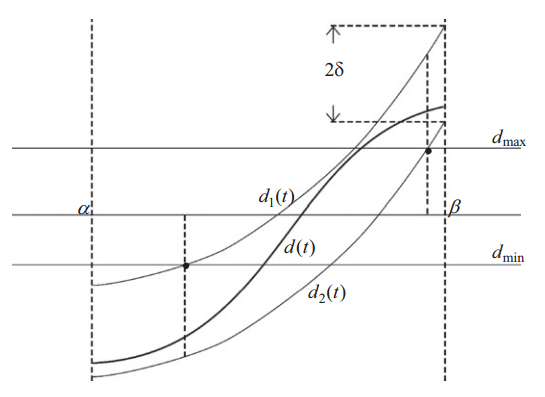
\includegraphics[width=0.6\textwidth]{dist}
    \caption{}
  	\label{slika4}
\end{figure}